\documentclass[12pt, oneside]{book}

\usepackage[]{graphicx}
\usepackage[]{color}
\usepackage{alltt}
\usepackage[utf8]{inputenc}
\setcounter{secnumdepth}{3}
\setcounter{tocdepth}{3}
\setlength{\parskip}{\smallskipamount}
\setlength{\parindent}{0pt}

\usepackage{DejaVuSans}
\renewcommand*\familydefault{\sfdefault}
\usepackage[T1]{fontenc}

\usepackage[top=50pt,bottom=50pt,left=68pt,right=66pt]{geometry}

\raggedbottom

\usepackage[portuguese]{babel}

\usepackage{fancyhdr}
\fancyhf{} 
\fancyfoot[C]{\thepage}
\renewcommand{\headrulewidth}{0pt} 
\pagestyle{fancy}

\fontfamily{DejaVu Sans Mono}\selectfont

\usepackage{titlesec}
\titleformat{\chapter}
   {\normalfont\LARGE\bfseries}{\thechapter.}{1em}{}
\titlespacing{\chapter}{0pt}{5pt}{1\baselineskip}

\usepackage{float}
\floatstyle{plaintop}

\usepackage[table]{xcolor}
\definecolor{lightgray}{gray}{0.9}

% descomente as linhas abaixo para não quebrar páginas entre capítulos
% uncomment the lines bellow to not break page between chapters
%\usepackage{etoolbox}
%\makeatletter
%\patchcmd{\chapter}{\if@openright\cleardoublepage\else\clearpage\fi}{}{}{}
% end page break configuration

\usepackage{hyperref}
\hypersetup{hidelinks,linkcolor = black}

\usepackage{background}
\usepackage{pdfpages}

\graphicspath{ {images/} }

\frontmatter

\backgroundsetup{
	scale=1,
	color=black,
	opacity=0.7,
	angle=0,
	contents={
		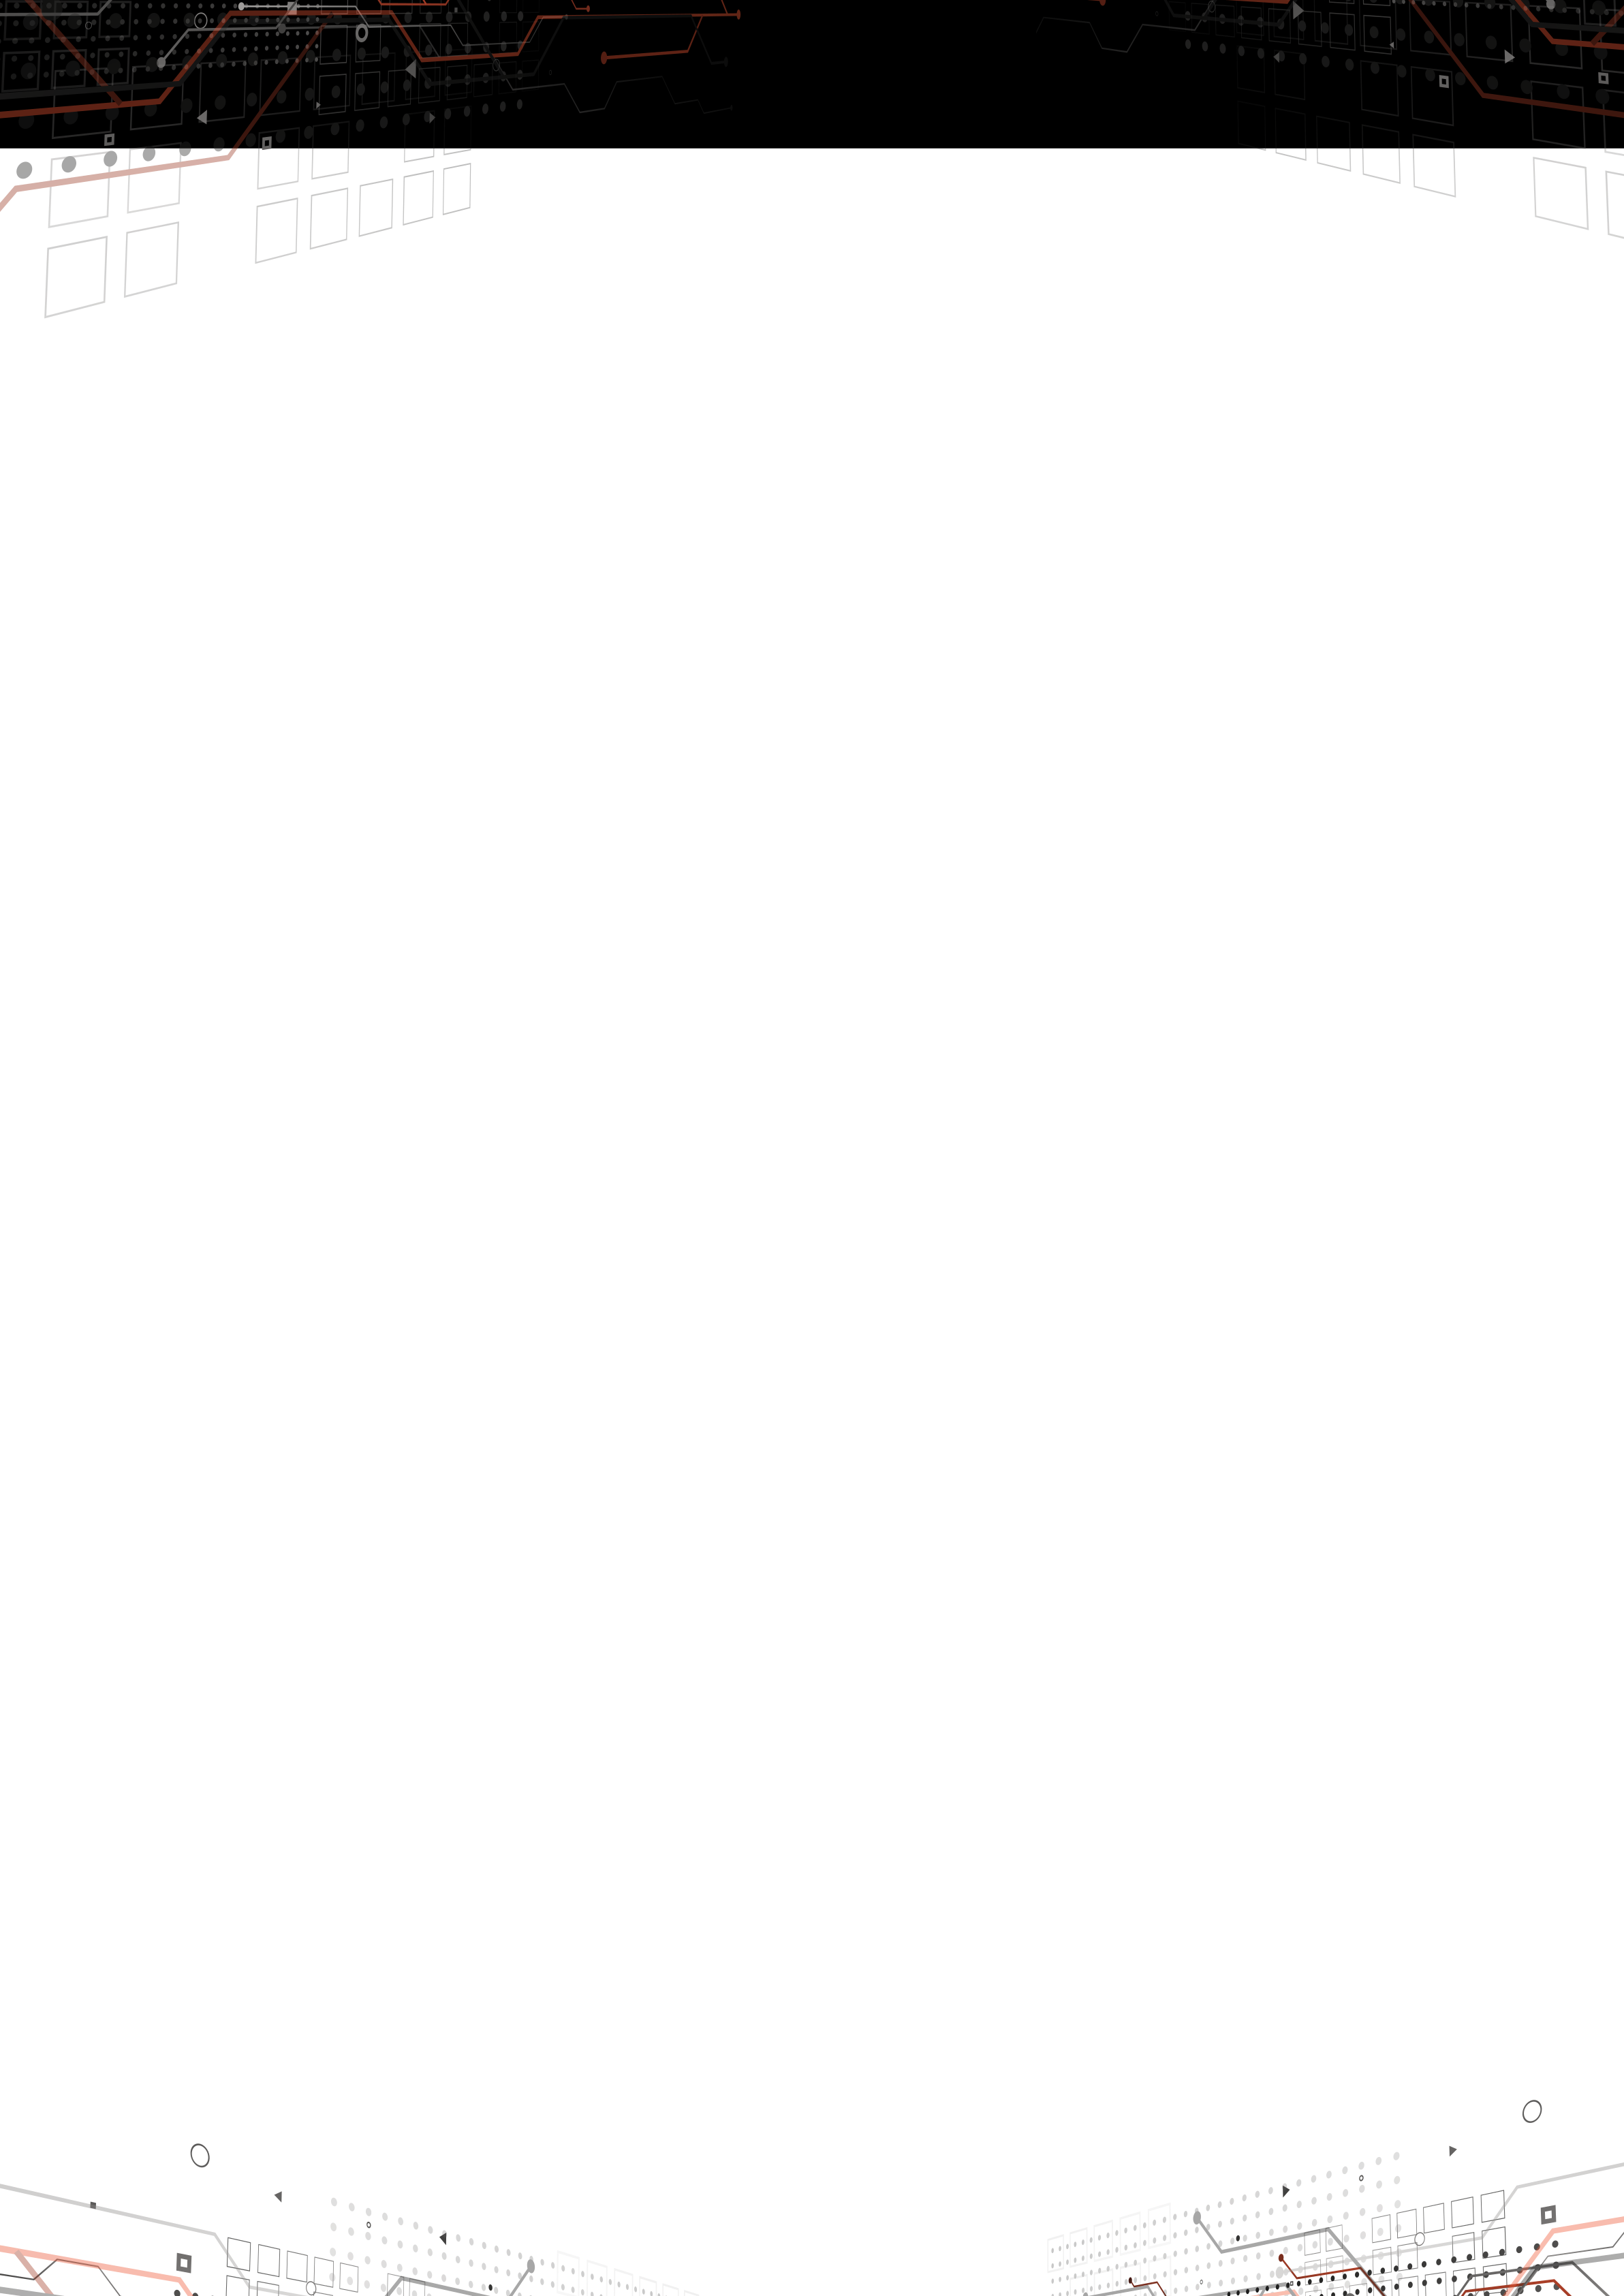
\includegraphics[width=\paperwidth,height=\paperheight]{images/header.png}
	}
}

\begin{document}

\selectlanguage{portuguese}

\begin{titlepage}
    \backgroundsetup{
        scale=1,
        color=black,
        opacity=1,
        angle=0,
        contents={
            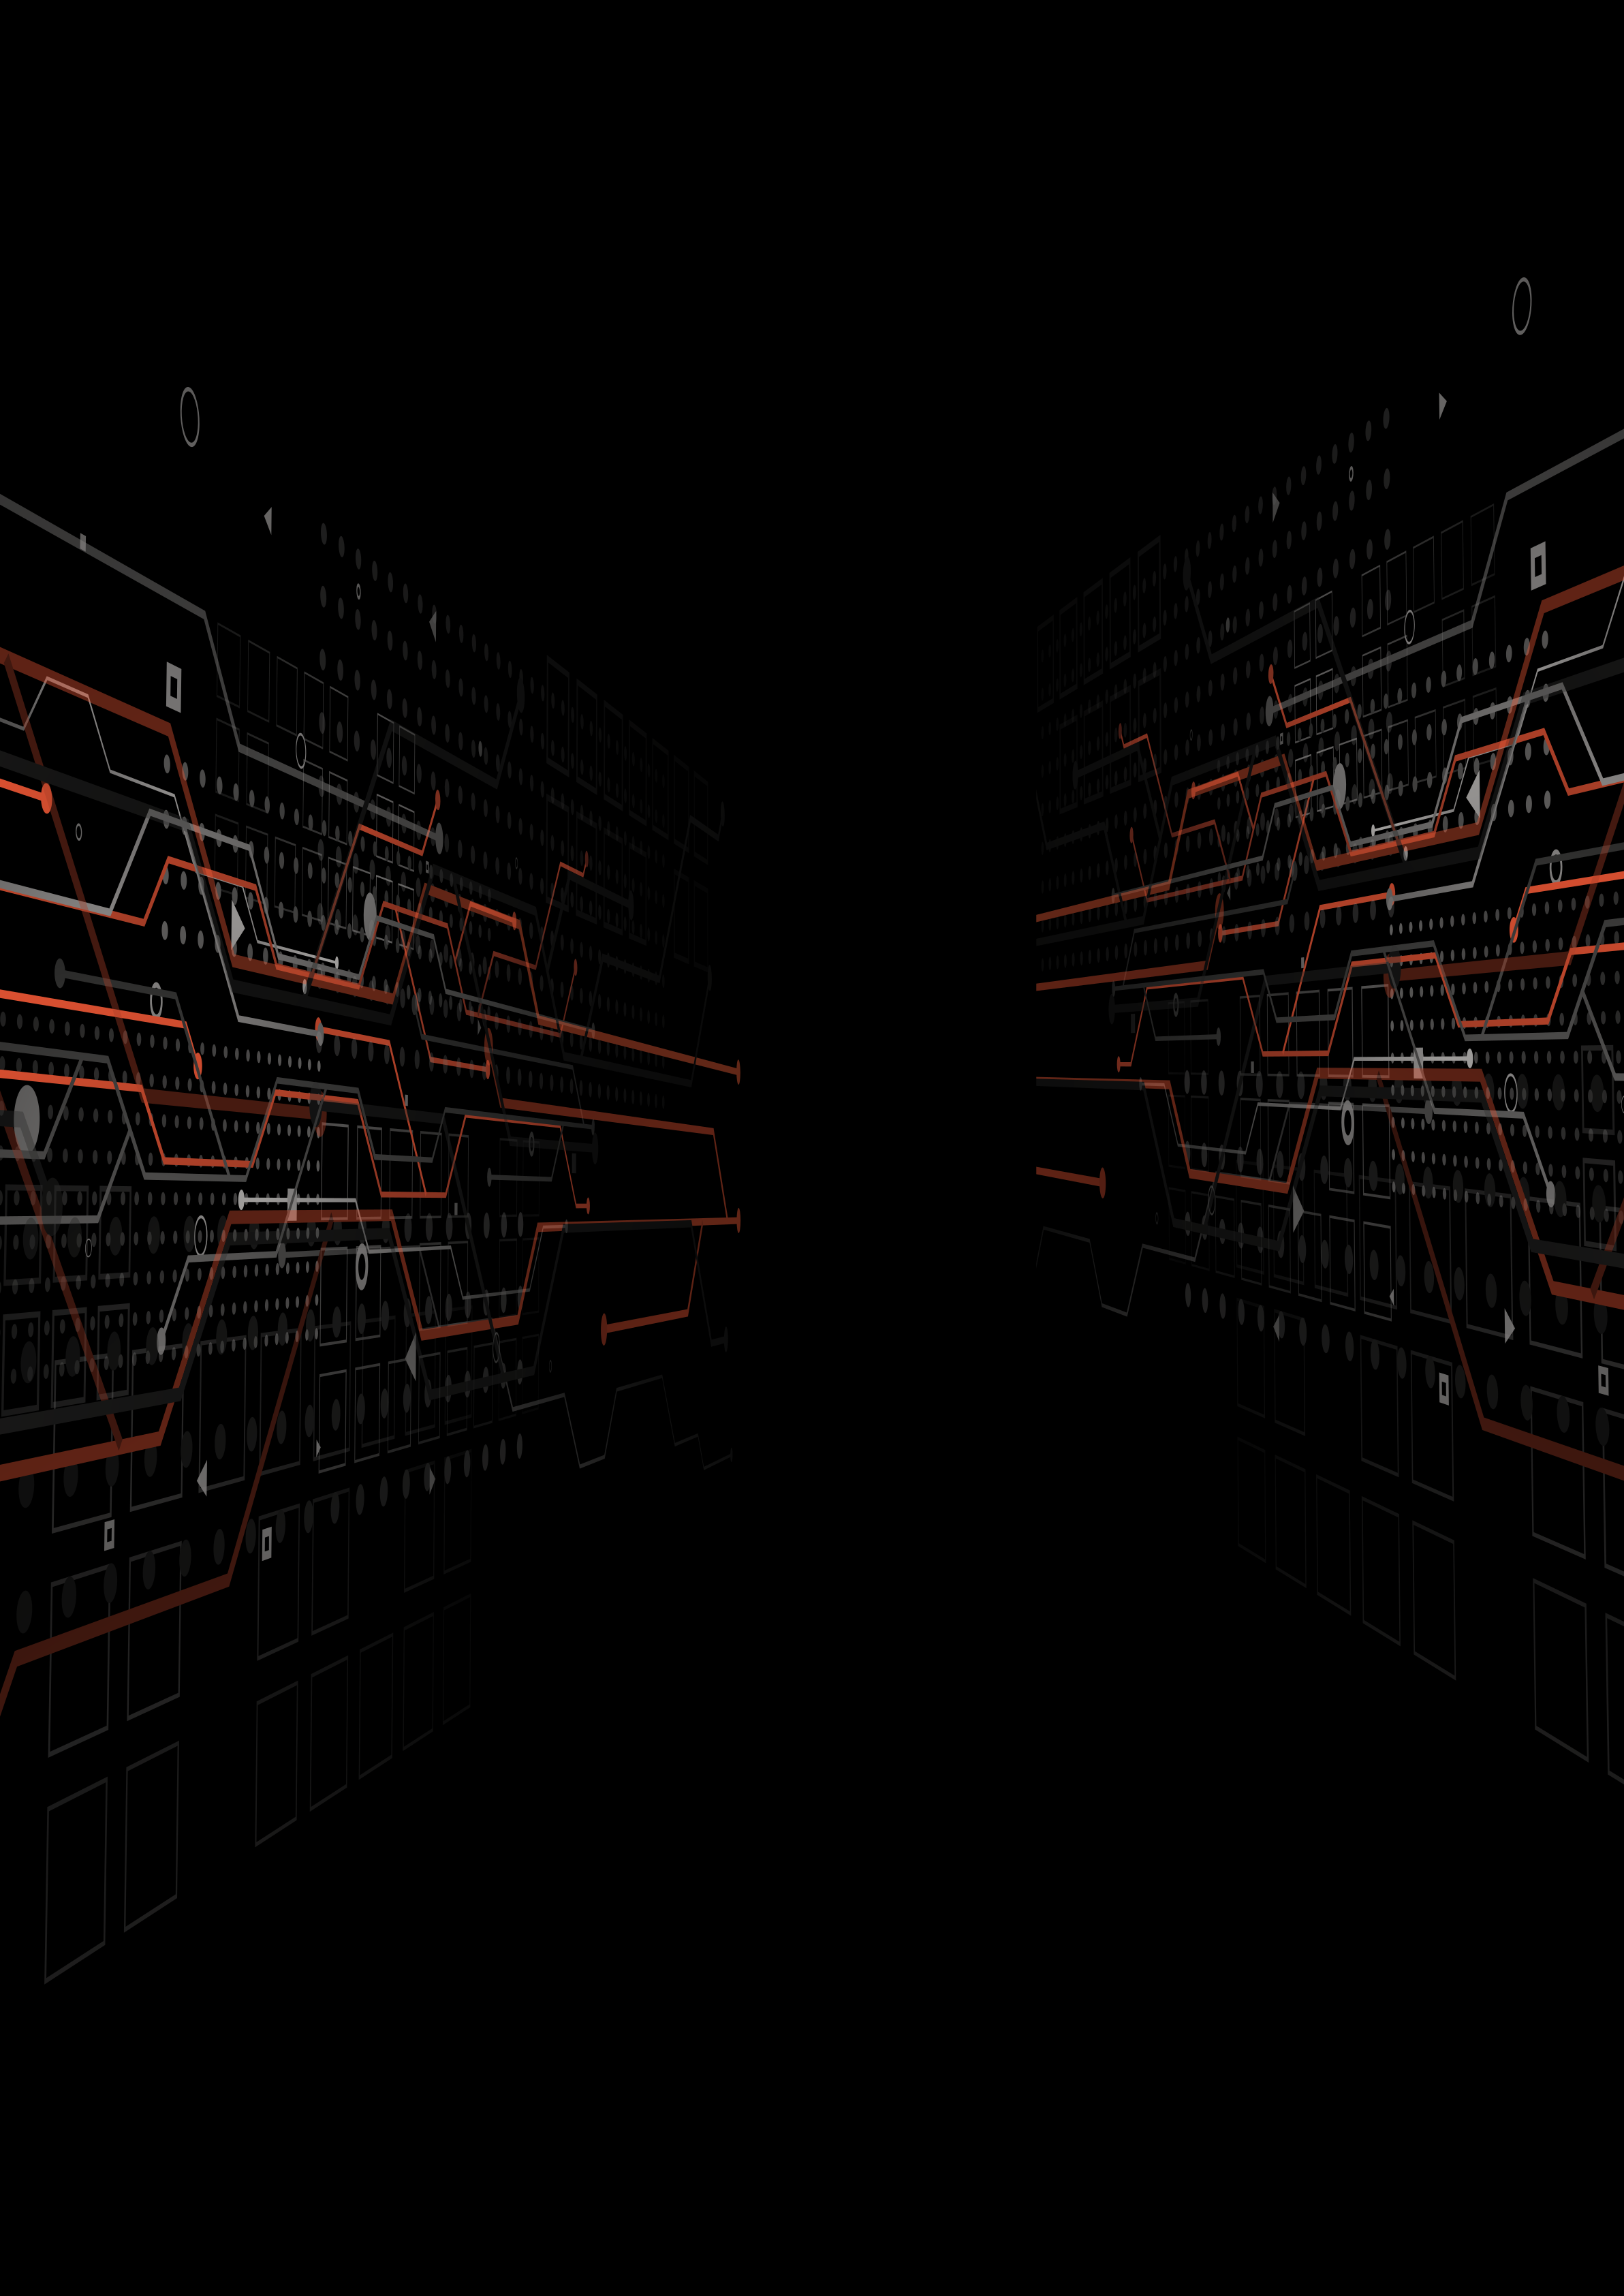
\includegraphics[width=\paperwidth,height=\paperheight]{images/background.png}
        }
    }

	\centering
    \color{white}

	\vspace{2cm}

	DOCUMENTO CONFIDENCIAL / CONFIDENTIAL DOCUMENT\par

    \vspace*{\fill}
	\vspace{4cm}
	\hrule
	\vspace{1cm}
	{\Huge \textbf{Nome do Projeto / Project Name}} \\
	\vspace{1cm}
	{\Large \textbf{Relatório de Pentest / Pentest Report}} \\
	\vspace{1cm}
	\hrule 
	\vspace{4cm}
	{\normalsize
		Gildásio Júnior
	}
	\vspace{2cm}

    \vspace{2cm}
    
	{\normalsize Salvador - BA\par}
	
	% {\normalsize XX-XX-20XX \par}	
	{\normalsize \today \par}
	\vspace{2cm}
	
	\pagebreak

\end{titlepage}

\newpage

\chapter{Grau de Sigilo / Secrecy Degree}

Esse é um documento \textbf{CONFIDENCIAL} e sua visualização é permitida apenas
à \textbf{EMPRESA}, contratante do consultor \textbf{Gildásio Júnior}. O acesso
por pessoa não autorizada poderá implicar em pena perante as leis.

This is a confidential document and its visualization is only allowed to
\textbf{COMPANY}, who hired the consultant \textbf{Gildásio Júnior}. The access
by non allowed person may result in penalties under the laws.

\newpage

\tableofcontents{}
\clearpage
\mainmatter

%%%%%%%%%%%%%%%%%%%%%%%%%%%%%%%%%%%%%%%%%%%%%%%%%%%%%%%%%%%%%%%%%%%%%%%%
% Include content
%%%%%%%%%%%%%%%%%%%%%%%%%%%%%%%%%%%%%%%%%%%%%%%%%%%%%%%%%%%%%%%%%%%%%%%%

\chapter{Título de Capítulo / Chapter Title}

Exemplo de citação / Citation example: \cite{reporttemplate}.

\section{Título de Seção}
\section{Section Title}

\pagebreak

%\appendix




\bibliographystyle{plain}
\bibliography{refs}
\addcontentsline{toc}{chapter}{\bibname}

\newpage
\vspace*{\fill}
\color{white}
\begin{flushright}
    \textbf{
        Gildásio Júnior \\
        email@provider \\
        +55 CellPhone \\
        gildasio.gitlab.io
    }
\end{flushright}

\backgroundsetup{
    scale=1,
    color=black,
    opacity=1,
    angle=0,
    contents={
        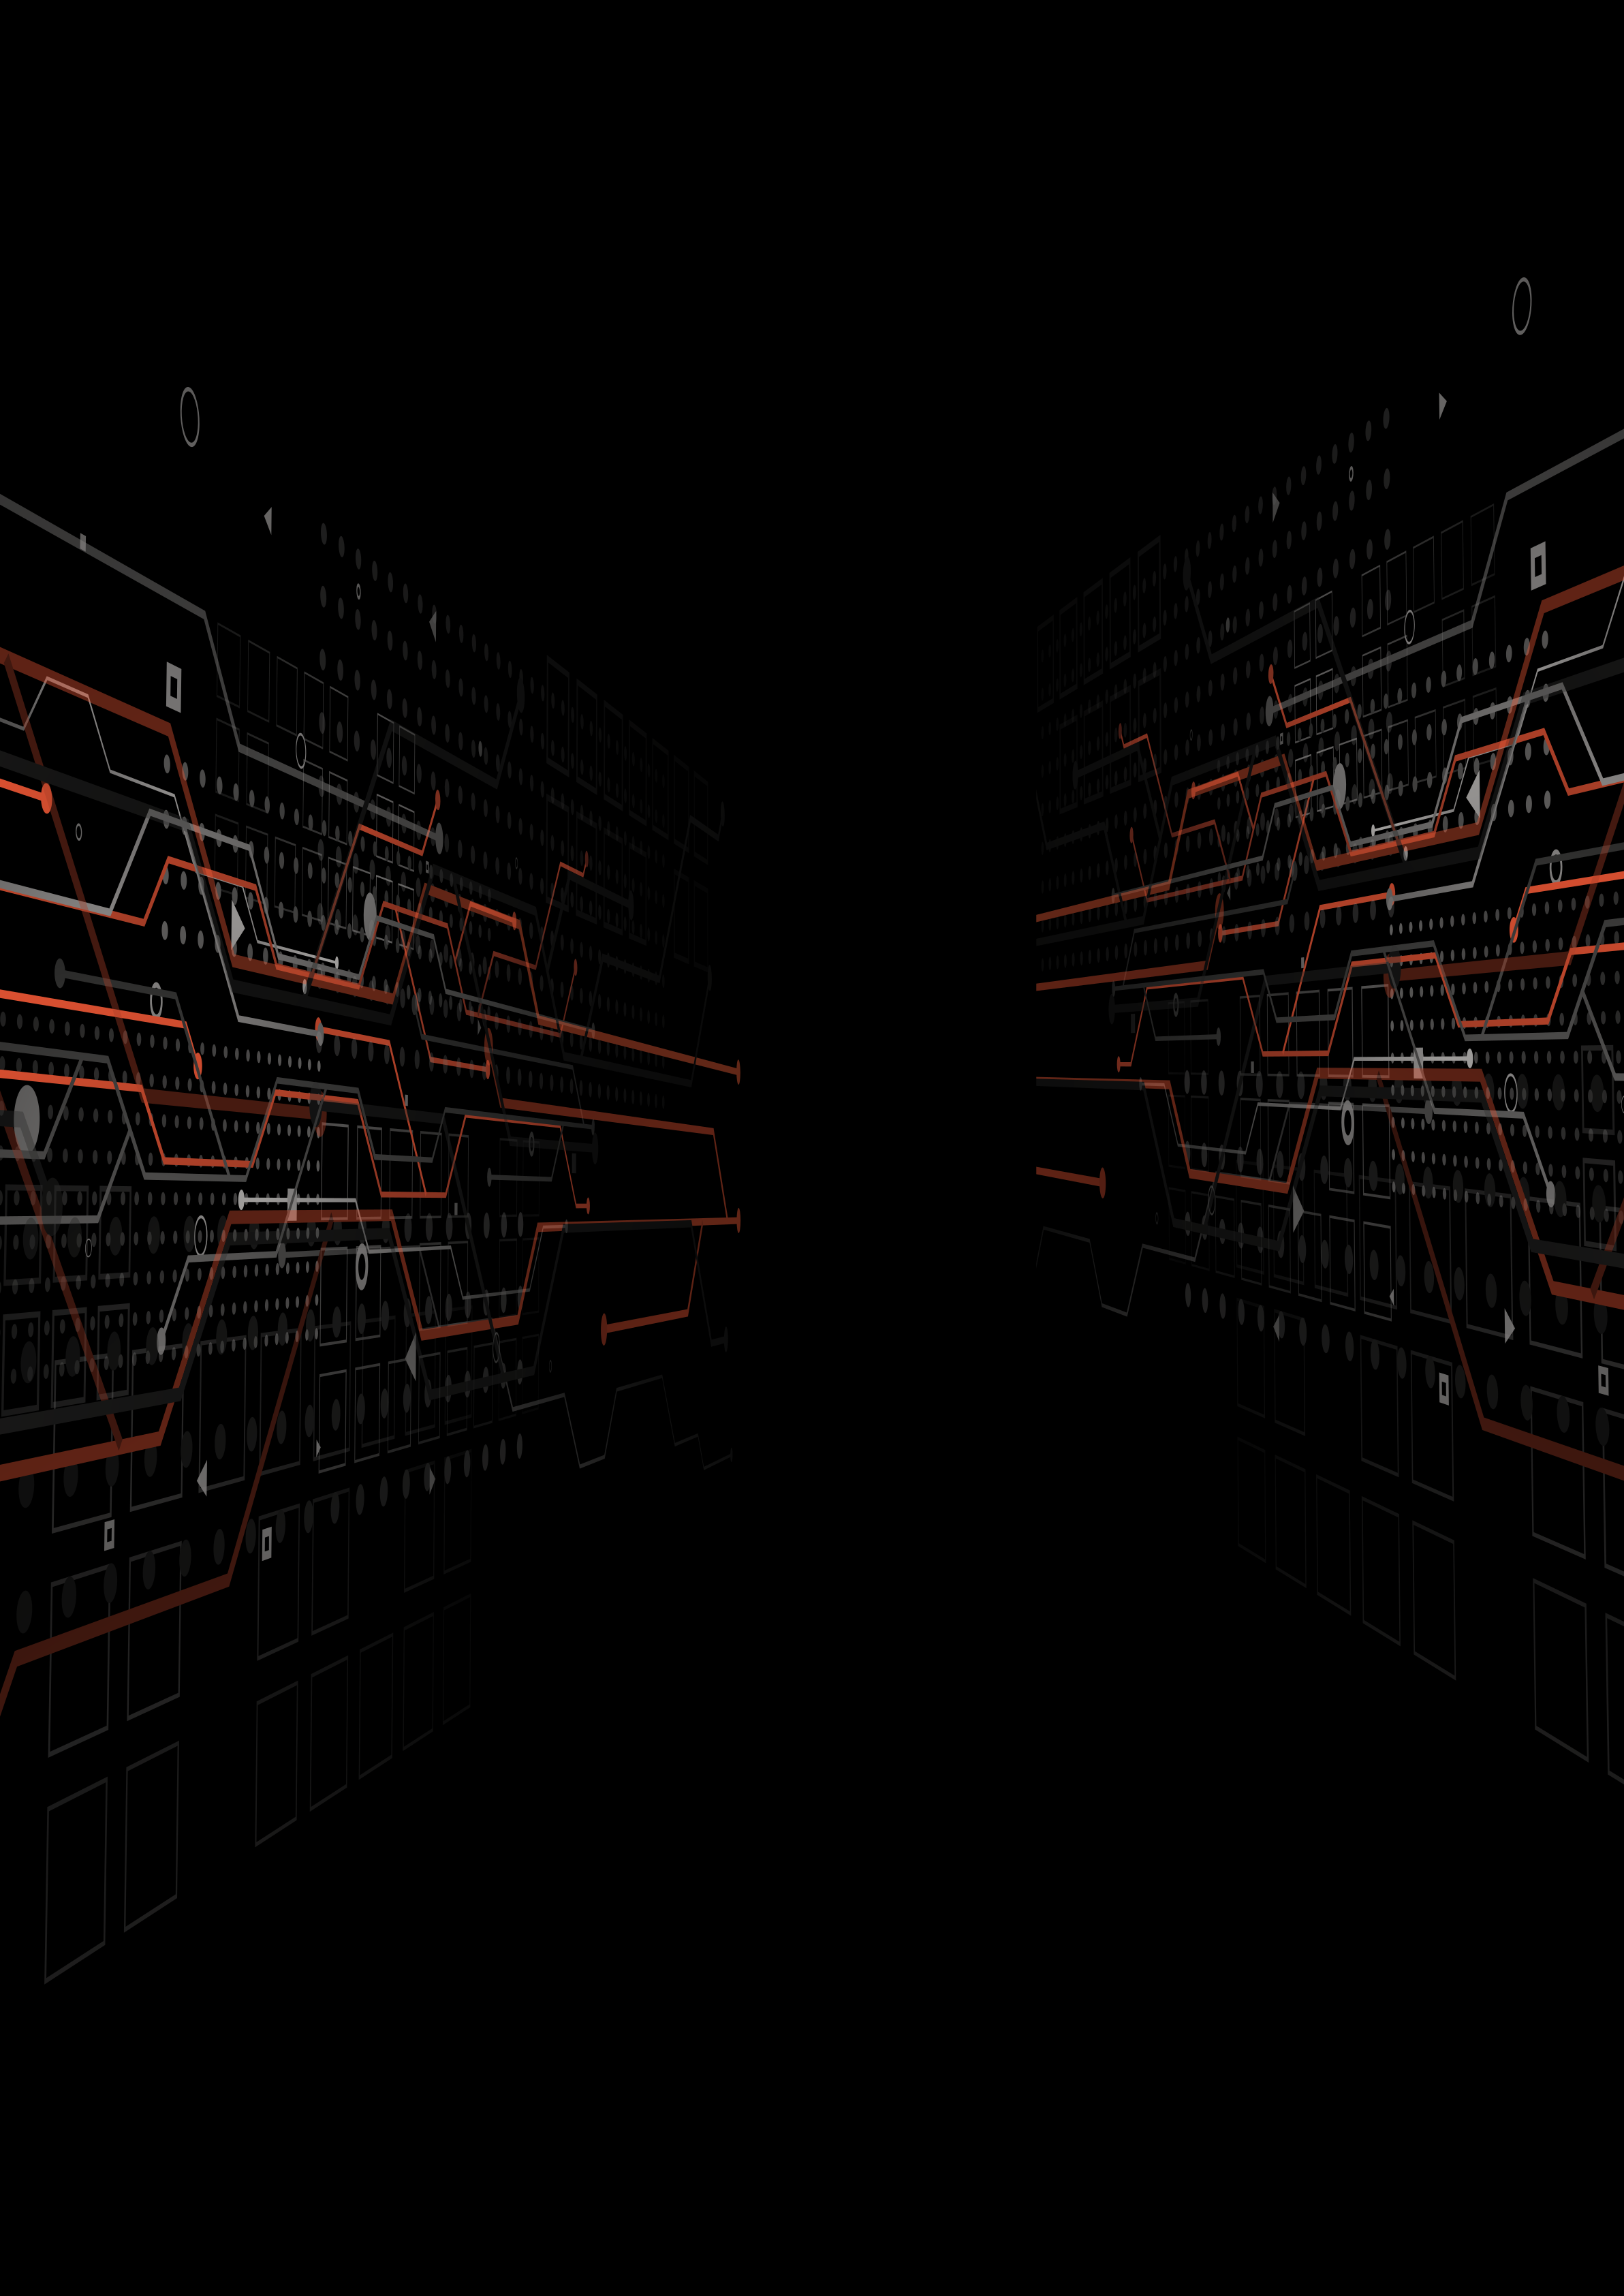
\includegraphics[width=\paperwidth,height=\paperheight]{images/background.png}
    }
}

\end{document}
